\documentclass{beamer}

\mode<presentation>
{
  \usetheme{Berlin}
  \setbeamercovered{transparent}
}

\setbeamertemplate{navigation symbols}{}


\usepackage[slovene]{babel}

\usepackage[latin1]{inputenc}
\usepackage{listings}

\usepackage{times}
\usepackage[T1]{fontenc}

\newcommand{\bx}{\mathbf{x}}
\DeclareMathOperator{\Gl}{Gl}
\DeclareMathOperator{\adj}{adj}
\newtheorem{proposition}[theorem]{Proposition}


\title[]
{Paralelizacija grafovskih algoritmov v funkcijskih jezikih}

\author[]
{Avtor: Tja\v z Er\v zen, Mentor: doc. dr. Matija Pretnar}


\date[12. december 2022] % (optional)
{Kratka predstavitev pri Diplomskem seminarju, 12. december 2022}


\begin{document}

\begin{frame}
  \titlepage
\end{frame}

\begin{frame}
  \frametitle{Uvod}
  \tableofcontents
\end{frame}

\section{Zakaj porazdeljeni sistemi?}

\begin{frame}{Uvod}
    \begin{itemize}
        \item Hitro ni dovolj hitro?
        \begin{itemize}
            \item Dana\v snji ra\v cunalniki so 100-krat hitrej\v si od tistih izpred desetletja, vendar sama ra\v cunska mo\v c pogosto ni dovolj.
            \item Dana\v snji ra\v cunalniki imajo bistveno ve\v c spominskih kapacitet od tistih izpred desetletja, vendar sama kapaciteta spomina pogosto ni dovolj.
        \end{itemize}
    \end{itemize}
\end{frame}

\begin{frame}{Uvod}
    \begin{itemize}
        \item Veliki izzivi ``large-scale'' sistemov:
        \begin{itemize}
            \item Ra\v cunalni\v sko-matemati\v cni problemi (npr. mno\v zenje matrik).
            \item Podatkovna analitika (ve\v cinoma gre za paralelizacijo na grafi\v cnih karticah)
            \item Modeliranje vremena in obna\v sanje okolja
            \item Ra\v cunsko te\v zki ra\v cunski problemi v fiziki in biologiji
            \item ...
        \end{itemize}
    \end{itemize}
\end{frame}

\begin{frame}{Je vzporedno programiranje sistemov res neizogibno?}
    \begin{itemize}
        \item Zmogljivej\v se sisteme trenutno dobimo predvsem z mno\v zenjem gradnikov
        \item Tehnologija izdelave \v cipov po\v casi zadeva ob oviro - bo Moorov zakon zdr\v zal?
        \begin{itemize}
            \item Do leta 2005 $50\%$ pove\v canje tranzistorjev vsako leto ($60$x v $10$ letih)
            \item Danes $20\%$ pove\v canje tranzistorjev vsako leto ($6$x v $10$ letih)
        \end{itemize}
        \item Nastane potreba po druga\v cnem na\v cinu optimizacije
    \end{itemize}
\end{frame}

\begin{frame}{Je vzporedno programiranje sistemov res neizogibno?}
    \begin{figure}[h!]
    \centering
    \caption{Fizikalno - ve\v cje oddajanje toplote v monolitnih kot v porazdeljenih sistemih}
    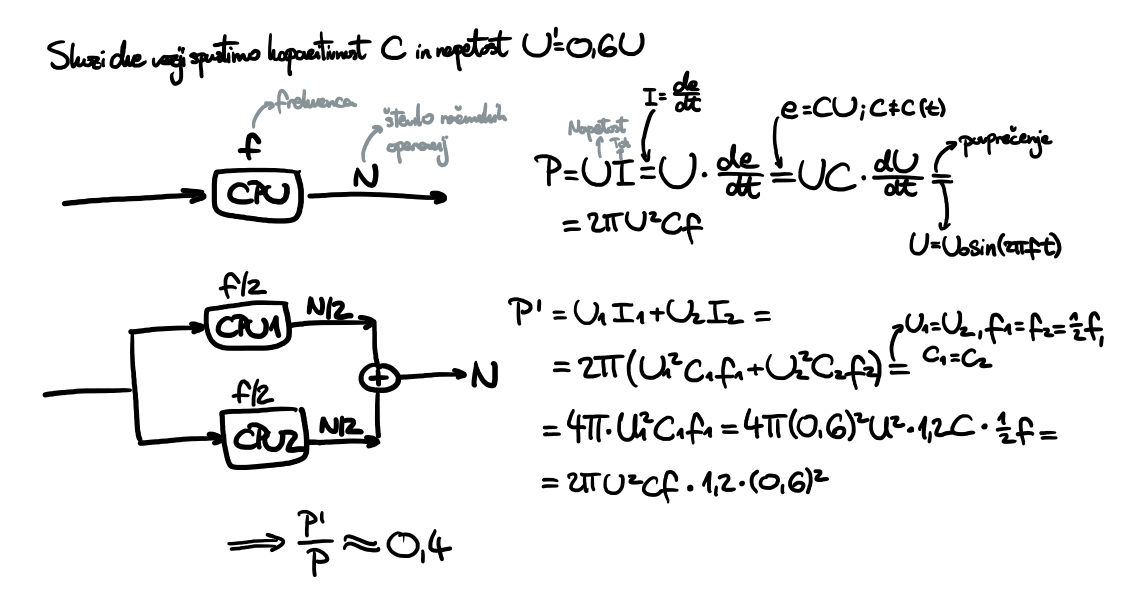
\includegraphics[width=10cm]{slike/paralelizacija-fizikalno.png}
    \label{fig:paralelizacija-fizikalno}
    \end{figure}
\end{frame}

\begin{frame}{Cilj paralelnega programa}
    Nekatere podatkovne strukture se da paralelizirati, medtem ko se drugih ne.
    \begin{figure}
    \caption{Paralelni programi so z ve\v canjem stevila jeder hitrej\v si.}
    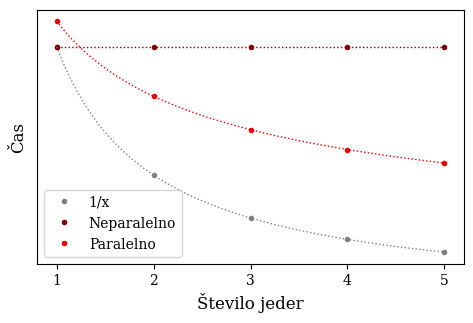
\includegraphics[width=6cm]{slike/cilj-casovne-zahtevnosti-paralelizacije.png}
    \label{fig:cilj-casovne-zahtevnosti-paralelizacije}
    \end{figure}
\end{frame}

\section{OCaml}

\begin{frame}{OCaml}
    \begin{itemize}
        \item Funkcijski jezik
        \item Leto\v snja razli\v cica verzije \textit{5.0.0}, ki (med drugim) vpelje knji\v znico za delo z vzporednimi procesi.
    \end{itemize}
    
    \begin{figure}
    \caption{Paralelizacija ra\v cunanja Fibonaccijevih \v stevil v OCamlu}
    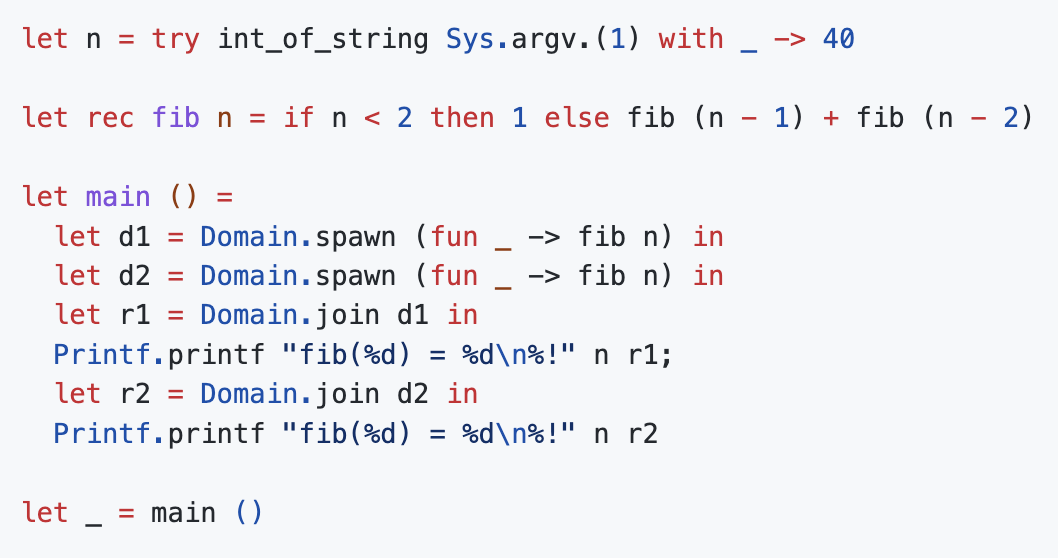
\includegraphics[width=6cm]{slike/OCaml-primer.png}
    \label{fig:OCaml-fibonacci}
    \end{figure}

\end{frame}


\section{Moja diplomska naloga}

\begin{frame}{Zakaj pisati vzporedne programe?}
    \begin{itemize}
        \item U\v cinkovitost
        \item Dobra novica: Potrebno znanje paralelizacije ra\v cunalni\v skih sistemov
        \item Slaba novica: Razvoj prevajalnikov, ki bi znali na\v se zaporedne programe samostojno pretvoriti v vzporedno obliko. Ideja: I\v s\v cejo se tipi\v cni programski konstrukti, ki se jih pretvarja v paralelno obliko
    \end{itemize}
\end{frame}

\begin{frame}{Cilji diplomske naloge}
    \begin{itemize}
        \item Paralelizacija ra\v cunalni\v skega procesorja v funkcijskem jeziku OCaml
        \item Se spoznati s paralelizacijo funkcijskih jezikov
        \item Pregled \v ze obstoje\v cih paralelnih knji\v znic v drugih funkcijskih jezikih (npr. Haskell) in implementacija le-teh v OCamlu
        \item Analiza podatkovnih struktur in algoritmov, primernih za paralelizacijo
    \end{itemize}
    
\end{frame}

\begin{frame}{Za\v cetni plan}
    \begin{itemize}
        \item Implementacija osnovnih matemati\v cnih funkcij z ``naivno'' paralelizacijo (\textit{map, apply, sum, ...})
        \item Ugotoviti, kdaj se nekaj spla\v ca paralelizirati in kdaj ne
        \item Implementacija/ razvoj manj trivialnih paralelnih algoritmov (grafi)
    \end{itemize}

\end{frame}

\end{document}